%% ============================================================================
%%  Journal version (Elsevier elsarticle).
%%  Compile order: pdflatex -> bibtex -> pdflatex -> pdflatex
%%  Overleaf: upload this file, refs.bib and the figures/ folder.
%% ============================================================================
\documentclass[preprint,12pt]{elsarticle}

\usepackage{amsmath,amssymb}
\usepackage{graphicx}
\usepackage{booktabs}
\usepackage{multirow}
\usepackage{url}
\usepackage{mathptmx}  % Times 系列，接近 Elsevier 正式排版
\usepackage{lineno}

\journal{Neurocomputing}

\newcommand{\ours}{\textsc{PAA}}
\newcommand{\ie}{i.e.}
\newcommand{\eg}{e.g.}

\begin{document}
\setlength{\emergencystretch}{1.5em}
\linenumbers


\begin{frontmatter}

\title{When Does Full Fine-Tuning Fail? A Cross-Backbone Study of Visual
Adaptation under Label Scarcity}

\author[a]{Jiahao Wu\corref{cor1}}
\ead{202531123002081@stu.hubu.edu.cn}
\author[a]{Sihao Li}

\cortext[cor1]{Corresponding author.}

\address[a]{Hubei University, Wuhan, Hubei, China}

\begin{abstract}
Practitioners adapting a pretrained visual model with few labels must choose
between updating all weights and updating a small subset. Published comparisons
disagree, and the disagreement may come from the protocol rather than from the
methods. We report a controlled study of eight adaptation paradigms---zero-shot,
prompt learning (CoOp), linear probing, full fine-tuning, BitFit, LoRA, residual
adapters and a prototype-anchored variant (\ours)---on two datasets, five
backbones (CLIP ViT-B/16, supervised ViT-B/16 and ViT-S/16, ConvNeXt-T,
ResNet-50), three label budgets and three seeds, over 1{,}428 runs. The study has
two tuning regimes: every method at one shared learning rate, which is what most
published comparisons do, and the rate chosen per method on the validation split
from a grid of up to seven values.

The first regime reproduces the field's most striking claim. Full fine-tuning
collapses on the three transformer backbones, losing 8--69 points to the best
parameter-efficient method, while the two convolutional backbones lose at most
15. The second regime dissolves the effect. On EuroSAT every backbone lands
within 2.6 points of the best parameter-efficient method once the rate is tuned,
and the CLIP gap falls from 68.8 to 2.3 points. The cause is that the rate which
maximises accuracy moves with the architecture by one to two orders of
magnitude---$10^{-5}$ to $10^{-4}$ for full fine-tuning on a ViT,
$3\times10^{-4}$ to $10^{-3}$ on a CNN---whereas the parameter-efficient family
moves by 1.6--8.4 points across the whole grid. A single-rate comparison
therefore manufactures an architecture effect, which is a plausible account of
why the literature disagrees.

What survives tuning is the number of examples per class. Where the budget leaves
one image per class, no trainable method beats zero-shot, and full fine-tuning
stays 3--10 points behind the best parameter-efficient method. Elsewhere the
ordering within that family is stable, prompt learning is the weakest adapted
method under this protocol, and \ours\ is competitive but never significantly
better.
\end{abstract}

\begin{keyword}
parameter-efficient transfer learning \sep label scarcity \sep vision--language
models \sep empirical study \sep reproducibility
\end{keyword}

\end{frontmatter}

%% ============================================================================
\section{Introduction}

Most visual recognition systems now start from a frozen encoder. A model
pretrained on web-scale image--text pairs, such as CLIP \cite{radford2021clip},
already separates many semantic categories it was never trained on, and a linear
probe on its features is a cheap and surprisingly strong baseline. For a target
domain close to the pretraining distribution this is usually enough.

It stops being enough when the domain is genuinely different and the labelling
budget is small. Satellite imagery, dermatoscopic photographs, leaf images taken
in the field, texture swatches: none of these are well represented in web-crawled
image--text data, so zero-shot inference and linear probing both leave a visible
gap. Something has to be adapted. The options are familiar. Unfreeze the whole
network, unfreeze only the biases, add low-rank updates, add bottleneck adapters,
or train a prompt.

\subsection{Why the choice is hard}

Two things make this choice harder than it should be.

The first is methodological. Each method tends to be reported under its own
protocol, with its own datasets, label budgets, augmentation and hyperparameter
search. Numbers that sit side by side in a related-work section are often not
comparable, and a method that received a wider search is difficult to tell apart
from a method that is simply better.

The second is substantive. The field has not settled whether full fine-tuning
helps or hurts when labels are scarce. One line of work shows that fine-tuning
distorts pretrained features and can end up worse than a linear probe out of
distribution \cite{kumar2022finetuning}, and proposes remedies that constrain or
interpolate the update \cite{wortsman2022wiseft}. Another line points the other
way: across many architectures and target datasets, fine-tuning the whole network
outperforms linear evaluation of the same frozen features
\cite{kornblith2019transfer}, which is one reason full fine-tuning remains the
default in transfer practice. Both cannot be right as stated for every model. The
two can both be right if the outcome depends on which model is being adapted, and
that is the possibility we test.

Our reading is that much of the disagreement comes from the protocol rather than
from the backbone: a large contrastively trained model and a smaller supervised
one need not respond to a few hundred gradient steps in the same way, and a
protocol that treats them identically can therefore report opposite conclusions
from the same data. We test this by running the grid twice, once with one shared
learning rate and once with the rate chosen per method.

\subsection{Contributions}

Our contributions are the following.

\begin{enumerate}
\item A controlled comparison in two tuning regimes: eight adaptation paradigms
on five backbones, two datasets, three label budgets and three seeds, 1{,}428
runs in total. One regime fixes the learning rate for every method; the other
selects it per method on the validation split. Code, splits and every
configuration are released, and we regard the grid rather than any single cell of
it as the object of the paper.

\item Evidence that the widely reported collapse of full fine-tuning on
transformer backbones is an artefact of the fixed rate. In the shared-rate
regime the three transformer backbones lose 8--69 points to the best
parameter-efficient method; with the rate chosen per method, every backbone on
EuroSAT lands within 2.6 points of it, and the CLIP gap falls from 68.8 to 2.3.
We designed this study expecting the opposite and report the correction in
\S\ref{sec:collapse}.

\item A quantification of the mechanism: the accuracy-maximising rate moves with
the architecture by one to two orders of magnitude ($10^{-5}$--$10^{-4}$ for full
fine-tuning on a ViT, $3\times10^{-4}$--$10^{-3}$ on a CNN), and full fine-tuning
is by far the most rate-sensitive family, spanning 45--80 points across the grid
where the parameter-efficient methods span 1.6--8.4. Any single-rate comparison
therefore carries a systematic bias of tens of points, which is a plausible
account of the field's disagreement.

\item Evidence that the number of examples per class, rather than the label
fraction, governs whether adaptation is worth attempting at all, and that this is
where full fine-tuning genuinely remains behind: where the budget leaves one
image per class, no trainable method beats zero-shot, and full fine-tuning stays
3--10 points below the best parameter-efficient method.

\item Evidence that the ordering within the parameter-efficient family (adapter
and LoRA above BitFit above a linear probe) is stable wherever adaptation
succeeds, and that prompt learning is the weakest adapted method under this
protocol.

\item \ours, a prototype-anchored adapter, evaluated like every other entry in
the grid: with the rate tuned it is the best entry in three of fourteen cells and
second in six, its largest deficit is 3.7 points, and the single significant
paired difference in the grid goes against it. We report its component ablation
and its cost, and we make no claim that it is the best method in this regime.
\end{enumerate}

The last point deserves emphasis. We began this work intending to propose a
method, and the experiments do not support a claim of superiority. What they do
support is a set of conditional statements about when each paradigm is
appropriate. We therefore report the study as an empirical one, and we report the
negative results alongside the positive ones.

%% ============================================================================
\section{Related Work}

\subsection{Frozen encoders and transfer with few labels}

CLIP \cite{radford2021clip} trains an image encoder and a text encoder to agree
on roughly four hundred million image--text pairs, and that agreement is what
makes zero-shot classification possible: embed the class names, embed the image,
take the closest. The vision transformer behind such models
\cite{dosovitskiy2021vit} has largely displaced convolutional networks here,
though ResNet \cite{he2016resnet} remains the reference architecture whenever
compute or latency matters.

Kornblith et al. \cite{kornblith2019transfer} found that ImageNet accuracy
predicts transfer accuracy across sixteen architectures and twelve datasets.
Their result is often read as permission to study a single strong backbone. It
also cuts the other way: if accuracy on the source task predicts accuracy after
transfer, then conclusions drawn from one architecture are only as general as
that architecture. With few labels per class, prototype classifiers
\cite{snell2017prototypical} are a natural fit, since class means stay stable
when the counts are small.

\subsection{Adapting without retraining everything}

The parameter-efficient family began with adapters \cite{houlsby2019adapter},
small bottleneck modules inserted into a frozen network, originally for language
models. LoRA \cite{hu2022lora} takes another route and factors the weight update
into two low-rank matrices. BitFit \cite{benzaken2022bitfit} goes further still
and trains only the bias terms. Prompt-based methods move the adaptation to the
input, in the text branch \cite{zhou2022coop} or in the visual token sequence
\cite{jia2022vpt}, while side-tuning \cite{zhang2020sidetuning} trains a separate
lightweight network that is summed with the frozen one.

One entry in our grid, \ours, sits in the adapter family. The two components it
adds are aimed specifically at the few-label regime, and they concern where the
classifier starts and how far the features are allowed to move. We describe them
in \S\ref{sec:method} and evaluate them alongside the other seven paradigms; no
result in this paper depends on the reader accepting them as an advance.

\subsection{The case against fine-tuning everything}

Kumar et al. \cite{kumar2022finetuning} showed that fine-tuning can distort
pretrained features badly enough to lose to a linear probe out of distribution,
and WiSE-FT \cite{wortsman2022wiseft} responds by interpolating fine-tuned and
zero-shot weights. Both point at the same idea: the adapted model should stay
close to the pretrained one. Our anchoring term applies that idea to
sample--prototype similarity rather than to weights, which means it needs no
weight averaging.

Kumar et al. \cite{kumar2022finetuning} also propose a two-stage remedy---a linear
probe followed by full fine-tuning---which is not among the paradigms we compare.
It is a plausible way to recover part of the gap we report, and we flag it as an
open question in \S\ref{sec:threats}.

What both papers share, and what we take as the opening for this work, is that
each studies a single backbone family. Neither varies the backbone as a
controlled factor, so neither can say whether the damage they document belongs to
fine-tuning or to the particular model being fine-tuned.

\subsection{Evaluation practice}

Our starting observation is narrower than the general complaint that evaluation
in the field is inconsistent. It is that, within a single comparison, methods
rarely receive the same optimiser settings and the same search budget, so a
method that received a wider search is difficult to distinguish from a method
that is better. Everything reported here sees the same images, the same
augmentation, the same schedule and the same seeds, with one deliberate
exception: every method is trained at the same learning rate, because that is
what most published comparisons do, and we measure the cost of doing so in
\S\ref{sec:lr}.

\section{Method}
\label{sec:method}

\subsection{Problem setting}

Let $f_\theta$ denote a frozen image encoder producing an embedding
$\phi(x) = f_\theta(x) \in \mathbb{R}^{d}$, and let
$\mathcal{D}_{\text{tr}} = \{(x_i, y_i)\}_{i=1}^{n}$ be a labeled training set
from a target domain with $C$ classes, where $n$ is deliberately small. We
consider adaptation procedures that introduce a set of trainable parameters
$\omega$ and a classifier $h_{\omega}: \mathbb{R}^d \to \mathbb{R}^C$. The
objective is accuracy on a held-out test set of the same domain. We treat $n$ as
the controlled variable and report the number of trainable parameters
$|\omega|$ alongside accuracy, because the two are the quantities a practitioner
actually trades off.

\subsection{Eight paradigms under one interface}

Seven of the eight methods share the interface ``feature extractor followed by a
cosine classifier'', so that only the adaptation mechanism varies; CoOp instead
leaves the image branch untouched and learns the text side, classifying by
image--text similarity. Both routes end in a cosine score over class embeddings,
which is what makes them comparable.

\emph{Zero-shot.} No training. Class logits are the cosine similarity between the
image embedding and the text embeddings of class names, using CLIP's text
encoder. Undefined for backbones without a text branch.

\emph{Prompt learning (CoOp).} Following \cite{zhou2022coop}, a set of $M$
learnable context vectors is prepended to the token embedding of each class name
and passed through the frozen text encoder; only the context vectors and the
logit scale are trained, and the image branch is frozen throughout. We use
$M=16$ and report it as a representative of the prompt-based family.

\emph{Linear probe.} $f_\theta$ is frozen and only $h_\omega$ is trained.

\emph{Full fine-tuning.} All parameters of the encoder and of the classifier are
trained. For CLIP this includes the text tower, which our implementation
unfreezes and which accounts for the 149.6M trainable parameters reported in
Table~\ref{tab:efficiency}; for the four ImageNet backbones it is the encoder
alone.

\emph{BitFit.} Only bias terms of $f_\theta$ and $h_\omega$ are trained
\cite{benzaken2022bitfit}.

\emph{LoRA.} Every adapted projection $W$ is replaced by
$W + \tfrac{\alpha}{r}BA$ with rank $r$ and $B$ initialized to zero
\cite{hu2022lora}.

\emph{Adapter.} A residual bottleneck is attached to each adapted projection,
$\mathrm{out} = Wx + U\,\sigma(Dx)$, with $U$ initialized to zero
\cite{houlsby2019adapter}.

\emph{\ours.} The adapter above, plus the two components described next.

Adapter and LoRA variants share the same injection points per backbone, so
differences between them reflect the update parameterization rather than the
placement.

\subsection{Prototype-anchored adapters}

\paragraph{Prototypical initialization}
Before training we compute class prototypes in the frozen feature space,
\begin{equation}
m_c = \frac{1}{n_c}\sum_{i:\,y_i=c} \phi(x_i),
\qquad c = 1,\dots,C,
\end{equation}
and initialize the classifier weights as $w_c = m_c/\lVert m_c\rVert$. The
logits are $s\cdot\cos(\phi(x), w_c)$ with a learnable scale $s$ initialized to
16. Starting from prototypes matters when $n$ is small: a randomly initialized
cosine classifier must first discover the geometry of the feature space, and
with a few dozen samples per class it often does not.

\paragraph{Prototype anchoring}
We allow the adapters to move features but penalize large deviations from the
frozen geometry. For a sample $(x_i,y_i)$ we add
\begin{equation}
\mathcal{L}_{\text{anchor}} = \frac{1}{n}\sum_{i}
\Bigl(1 - \cos\bigl(\tilde{\phi}(x_i),\, \hat{m}_{y_i}\bigr)\Bigr),
\end{equation}
where $\tilde{\phi}$ is the adapted feature and $\hat{m}$ the normalized
prototype of the ground-truth class. The total objective is
\begin{equation}
\mathcal{L} = \mathcal{L}_{\text{CE}} + \lambda\,\mathcal{L}_{\text{anchor}},
\end{equation}
with $\lambda = 0.5$ in every cell of the grid. We did not tune $\lambda$ per
cell, so any gain we attribute to the term is a lower bound on what tuning it
could buy. The term is one-sided: it discourages moving away from the class
prototype but does not prevent the adapter from rotating features to separate
confusable classes.

\paragraph{Expected effect and its limits}
Two effects are expected. First, the anchoring term keeps the adapted
representation close enough to the frozen one that the prototypical classifier
remains meaningful throughout training. Second, it acts as a data-dependent
regularizer whose strength scales with label scarcity. \S\ref{sec:ablation}
isolates both components on CLIP and finds that the anchoring term carries most
of the gain there; the cross-backbone results show that the second effect has a
precondition we did not anticipate, namely that there must be drift to
regularize.

\subsection{Optimization and cost}

All trainable methods use AdamW with weight decay, a cosine learning-rate
schedule without warm-up, and early stopping on a held-out validation subset; the
classifier receives a learning-rate multiplier of 10 relative to the encoder.
\ours\ costs no more than the adapter it is built on: at inference it has exactly
the adapter's parameters, because the prototypes are computed once before
training and the anchoring term vanishes afterwards.

%% ============================================================================
\section{Experimental setup}
\label{sec:setup}

\subsection{Datasets}

We use two datasets chosen to differ in label-space size and in the kind of
domain gap they present.

\emph{EuroSAT} \cite{helber2019eurosat} contains 27{,}000 Sentinel-2 patches of
$64\times64$ pixels covering ten land-use classes. It embodies a large domain
gap to web-crawled imagery: an unadapted CLIP model reaches only 32.1\% top-1
accuracy on it, although chance is 10\%.

\emph{DTD} \cite{cimpoi2014dtd} contains 5{,}640 images of 47 describable
texture categories. Textures are a visual modality that image--text pretraining
covers thinly, and the label space is nearly five times larger than that of
EuroSAT; zero-shot CLIP reaches 42.9\%. The two datasets therefore differ in
both the size of the label space and the accuracy headroom left to adaptation.

\subsection{Backbones}

The central variable of this study is the backbone, and we choose two that
differ in exactly the way the literature makes it hard to compare.

\emph{CLIP ViT-B/16} \cite{radford2021clip} is contrastively trained on roughly
four hundred million image--text pairs. Its features are wide and distributed,
and support zero-shot classification through text embeddings, which also gives
us a no-training baseline.

\emph{ViT-B/16, supervisedly pretrained.} The same architecture as CLIP's
vision tower---twelve transformer blocks, 86M parameters---trained on ImageNet-1k
with a supervised classification objective \cite{dosovitskiy2021vit}. It shares
architecture and parameter count with CLIP and differs only in the pretraining
objective, which makes it the control that separates those two factors. It has no
text encoder.

\emph{ViT-S/16, supervisedly pretrained.} A smaller transformer of the same
family (21.7M parameters, 384-dimensional features), supervisedly pretrained on
ImageNet-1k. Its role is to break the confound between architecture and
parameter count: it has fewer parameters than either convolutional backbone we
use, so if it still collapses the cause cannot be size.

\emph{ConvNeXt-T} \cite{liu2022convnext} and \emph{ResNet-50}
\cite{he2016resnet} are supervisedly trained on ImageNet-1k, with 28.6M and
25.0M parameters respectively. They provide the convolutional comparison at a
parameter count comparable to ViT-S/16. ConvNeXt is a modern convolutional
architecture that borrows several design choices from transformers while keeping
convolutions and a hierarchical feature pyramid, so the pair spans both an
older and a current convolutional design. Zero-shot inference is undefined for both and we report it as not
applicable rather than as a number.

All five backbones are used at $224\times224$ resolution. For the four
non-contrastive backbones we evaluate only the two scarce budgets, since the
question of the paper concerns that regime.

\subsection{Splits and label budgets}

For each dataset we create a stratified 80/10/10 train/validation/test split
with a fixed seed and keep the split file so that every method sees exactly the
same images. The splits contain 21{,}600 / 2{,}700 / 2{,}700 images for EuroSAT
and 4{,}512 / 564 / 564 for DTD. The budget is applied to the training split
only, per class, by keeping $k_c = \max(1, \mathrm{round}(\rho\, n_c))$ images of
class $c$, with $\rho \in \{1\%, 10\%, 100\%\}$. At $\rho=1\%$ this leaves 216
images for EuroSAT---about 22 per class, more for the larger classes, since the
ten classes are not exactly equal in size---and 47 for DTD, exactly one per
class, the smallest non-degenerate labelled set our protocol allows. Reported
accuracies always use the full test set, and the test set is never used for any
decision; early stopping uses the first 1{,}000 images of the validation split.

\subsection{Training settings}
\label{sec:training}

Adapter and LoRA injection targets are the query, key, value and output
projections and the two MLP projections of the vision transformer, the
convolutional blocks of the last residual stage for ResNet-50 (ten layers, so
that the parameter budget is comparable to the transformer case), and the
corresponding blocks of the last ConvNeXt stage. LoRA uses $r=8$, $\alpha=16$;
residual adapters use a bottleneck width of 32.

All methods train with AdamW, weight decay $0.05$, batch size 64 and a cosine
learning-rate schedule without warm-up, for at most 20 epochs (10 at
$\rho=100\%$), stopping early when validation accuracy has not improved for eight
epochs. The classifier head is trained at ten times the encoder learning rate.
Images are resized to $224\times224$ and augmented identically for every method.
$\lambda=0.5$ for \ours\ in every cell.

\paragraph{Two tuning regimes.} The grid is run twice, and the contrast between
the two runs carries most of the paper's argument.

In the \emph{shared-rate} regime every method is trained at $10^{-3}$. This is the
protocol most published comparisons use, so it is the one a practitioner actually
meets, and holding the rate fixed keeps the comparison internally uniform;
Tables~\ref{tab:eurosat}, \ref{tab:dtd}, \ref{tab:app-vits} and
\ref{tab:app-convnext} report it.

In the \emph{tuned} regime the rate for each (dataset, backbone, method, budget)
cell is the value with the highest mean validation accuracy over the three seeds,
taken from a per-method grid: $\{10^{-3}, 3\times10^{-4}, 10^{-4}\}$ for the
parameter-efficient methods and CoOp, $\{10^{-3}, 3\times10^{-4}, 10^{-4},
3\times10^{-5}, 10^{-5}\}$ for full fine-tuning, and additionally $\{3\times
10^{-3}, 10^{-2}\}$ for full fine-tuning on the two convolutional backbones. The
test set plays no part in the choice. The grids differ in size and full
fine-tuning's is the widest; we say so because a wider grid can only help that
method, which makes its remaining deficit on DTD (\S\ref{sec:onelabel}) the more
conservative estimate.

\subsection{Metrics and statistical testing}
\label{sec:metrics}

We report top-1 accuracy, macro-averaged accuracy, the number of trainable
parameters, and wall-clock training time on one NVIDIA RTX 5070~Ti laptop GPU.
Every configuration is run with three seeds (0, 1, 2), and means are reported
with standard deviations. The comparison in Table~\ref{tab:stats} is
additionally tested with a paired $t$-test. Two caveats govern how that test is
read: with three seeds it has $df=2$ and a two-sided critical value of 4.303, so
its power is low, and it treats seed-to-seed variation as the sampling unit,
which is not the same thing as method-to-method variation. We therefore use it as
a secondary check and take the primary evidence from the size of the differences
and their consistency in sign.

We also quantified run-to-run variation directly, by repeating twelve
configurations under identical settings. The mean absolute difference was 0.4
points and the largest 1.4. Differences below about one point---which includes
most of the ordering inside the parameter-efficient family---should be read as
within noise rather than as a ranking, and we interpret the tables accordingly.

%% ============================================================================
\section{Results}
\label{sec:results}

\subsection{Main comparison}

Tables~\ref{tab:eurosat} and~\ref{tab:dtd} report the shared-rate regime: top-1
accuracy on both datasets and three backbones, with every method at $10^{-3}$.
Reading down a column compares paradigms; across the blocks of a table, backbones.
The largest effects are in the third direction, and the rest of this section is
about what happens to them once the rate is tuned.

\begin{table}[t]
\centering
\caption{EuroSAT, shared-rate regime (every method at $10^{-3}$): top-1 accuracy
(\%) for three of the five backbones. Mean $\pm$ standard deviation over three
seeds. CLIP is evaluated at all three budgets; the two other backbones only at the
scarce budgets, since that is the regime the paper concerns. Zero-shot and prompt
learning are defined only for the image--text backbone; the dashes mark cells that
do not apply. The remaining two backbones are in \ref{app:extra}.}
\label{tab:eurosat}
\scriptsize
\setlength{\tabcolsep}{3.5pt}
\begin{tabular}{lccccccc}
\toprule
 & \multicolumn{3}{c}{CLIP ViT-B/16 (contrastive)} & \multicolumn{2}{c}{ViT-B/16 (supervised)} & \multicolumn{2}{c}{ResNet-50} \\
\cmidrule(lr){2-4}\cmidrule(lr){5-6}\cmidrule(lr){7-8}
Method & 1\% & 10\% & 100\% & 1\% & 10\% & 1\% & 10\% \\
\midrule
Zero-shot & -- & -- & 32.11 & n/a & n/a & n/a & n/a \\
CoOp & 80.17$\pm$0.33 & 89.28$\pm$1.22 & 92.41$\pm$0.32 & -- & -- & -- & -- \\
Linear probe & 82.83$\pm$0.80 & 90.95$\pm$1.20 & 94.22$\pm$0.52 & 88.01$\pm$1.23 & 93.91$\pm$0.45 & 81.14$\pm$0.86 & 90.32$\pm$0.48 \\
BitFit & 91.67$\pm$0.65 & 96.67$\pm$0.93 & 98.37$\pm$0.39 & 90.59$\pm$1.49 & 96.40$\pm$0.15 & 81.72$\pm$0.83 & 92.83$\pm$0.15 \\
LoRA & 93.07$\pm$1.17 & 96.95$\pm$0.74 & \textbf{98.84}$\pm$\textbf{0.15} & 90.96$\pm$0.77 & 97.09$\pm$0.41 & 85.84$\pm$1.59 & 95.36$\pm$0.37 \\
Adapter & 93.69$\pm$0.40 & 97.43$\pm$0.52 & 98.75$\pm$0.08 & 91.42$\pm$1.90 & 96.78$\pm$0.49 & 86.89$\pm$1.09 & 95.22$\pm$1.07 \\
\textbf{\ours} & \textbf{94.12}$\pm$\textbf{0.28} & \textbf{97.47}$\pm$\textbf{0.31} & 98.75$\pm$0.39 & \textbf{92.19}$\pm$\textbf{0.74} & \textbf{97.21}$\pm$\textbf{0.43} & 85.81$\pm$1.35 & 95.09$\pm$0.49 \\
Full FT & 25.30$\pm$4.26 & 51.04$\pm$12.25 & 70.77$\pm$5.09 & 33.90$\pm$1.39 & 78.40$\pm$3.54 & \textbf{87.14}$\pm$\textbf{1.06} & \textbf{97.07}$\pm$\textbf{0.23} \\
\bottomrule
\end{tabular}
\end{table}

\begin{table}[t]
\centering
\caption{DTD, shared-rate regime (every method at $10^{-3}$): top-1 accuracy
(\%). At $\rho=1\%$ the training subset contains exactly one image per class.
Same layout as Table~\ref{tab:eurosat}: three of the five backbones, CLIP at all
three budgets. The remaining two backbones are in \ref{app:extra}.}
\label{tab:dtd}
\scriptsize
\setlength{\tabcolsep}{3.5pt}
\begin{tabular}{lccccccc}
\toprule
 & \multicolumn{3}{c}{CLIP ViT-B/16 (contrastive)} & \multicolumn{2}{c}{ViT-B/16 (supervised)} & \multicolumn{2}{c}{ResNet-50} \\
\cmidrule(lr){2-4}\cmidrule(lr){5-6}\cmidrule(lr){7-8}
Method & 1\% & 10\% & 100\% & 1\% & 10\% & 1\% & 10\% \\
\midrule
Zero-shot & -- & -- & 42.91 & n/a & n/a & n/a & n/a \\
CoOp & 24.41$\pm$3.43 & 60.28$\pm$1.41 & 75.06$\pm$2.20 & -- & -- & -- & -- \\
Linear probe & 36.64$\pm$2.39 & 67.67$\pm$2.20 & 79.49$\pm$1.01 & 28.72$\pm$1.77 & 60.70$\pm$0.54 & 25.06$\pm$2.97 & 55.14$\pm$0.47 \\
BitFit & 38.48$\pm$2.65 & 70.80$\pm$1.33 & 82.09$\pm$0.64 & 29.55$\pm$3.80 & 63.30$\pm$1.11 & 25.18$\pm$3.15 & 55.08$\pm$0.54 \\
LoRA & 39.42$\pm$1.82 & 71.69$\pm$0.98 & 82.51$\pm$0.57 & 29.43$\pm$0.53 & 64.30$\pm$2.49 & 25.77$\pm$2.46 & 55.79$\pm$1.14 \\
Adapter & \textbf{39.60}$\pm$\textbf{1.79} & 68.91$\pm$1.18 & 82.33$\pm$0.57 & \textbf{31.50}$\pm$\textbf{2.84} & \textbf{64.54}$\pm$\textbf{1.85} & 25.18$\pm$1.92 & 58.10$\pm$2.02 \\
\textbf{\ours} & 39.07$\pm$1.08 & \textbf{71.93}$\pm$\textbf{1.13} & \textbf{83.10}$\pm$\textbf{0.72} & 30.32$\pm$2.04 & 63.59$\pm$2.25 & \textbf{25.95}$\pm$\textbf{1.72} & \textbf{58.22}$\pm$\textbf{2.20} \\
Full FT & 3.07$\pm$0.57 & 4.61$\pm$0.47 & 9.63$\pm$0.62 & 5.02$\pm$1.78 & 5.14$\pm$0.77 & 19.50$\pm$0.99 & 44.21$\pm$2.57 \\
\bottomrule
\end{tabular}
\end{table}

\subsection{The collapse is an artefact of the shared rate}
\label{sec:collapse}

This is the main result of the paper, and it is a negative one for the hypothesis
we set out to test. \S\ref{sec:training} described two regimes over the same cells;
Table~\ref{tab:collapse} puts them side by side.

\begin{table}[t]
\centering
\caption{Full fine-tuning against the best parameter-efficient method, under a shared learning rate ($10^{-3}$ for every method) and with the rate chosen per method on the validation split. $\Delta$ is full fine-tuning minus the best parameter-efficient method; negative means fine-tuning is worse. Bold marks a gap wider than 10 points.}
\label{tab:collapse}
\small
\setlength{\tabcolsep}{3pt}
\begin{tabular}{llcc ccc}
\toprule
 & & & \multicolumn{2}{c}{shared rate} & \multicolumn{2}{c}{tuned} \\
\cmidrule(lr){4-5}\cmidrule(lr){6-7}
Dataset & Backbone & $\rho$ & Full FT & $\Delta$ & Full FT & $\Delta$ \\
\midrule
EuroSAT & CLIP ViT-B/16 & 1\% & 25.3 & $\mathbf{-68.8}$ & 91.8 & $-2.3$ \\
EuroSAT & ViT-B/16 (sup.) & 1\% & 33.9 & $\mathbf{-58.3}$ & 91.7 & $-0.5$ \\
EuroSAT & ViT-S/16 (sup.) & 1\% & 45.8 & $\mathbf{-45.7}$ & 90.7 & $-0.7$ \\
EuroSAT & ConvNeXt-T & 1\% & 86.5 & $-5.8$ & 91.0 & $-1.3$ \\
EuroSAT & ResNet-50 & 1\% & 87.1 & $+0.2$ & 89.5 & $+2.6$ \\
\midrule
EuroSAT & CLIP ViT-B/16 & 10\% & 51.0 & $\mathbf{-46.4}$ & 97.1 & $-0.3$ \\
EuroSAT & ViT-B/16 (sup.) & 10\% & 78.4 & $\mathbf{-18.8}$ & 97.2 & $+0.1$ \\
EuroSAT & ViT-S/16 (sup.) & 10\% & 89.2 & $-8.0$ & 96.7 & $-0.5$ \\
EuroSAT & ConvNeXt-T & 10\% & 96.4 & $-0.8$ & 97.3 & $+0.1$ \\
EuroSAT & ResNet-50 & 10\% & 97.1 & $+1.7$ & 97.0 & $+1.6$ \\
\midrule
DTD & CLIP ViT-B/16 & 1\% & 3.1 & $\mathbf{-36.5}$ & 30.0 & $-9.6$ \\
DTD & ViT-B/16 (sup.) & 1\% & 5.0 & $\mathbf{-26.5}$ & 25.1 & $-6.4$ \\
DTD & ViT-S/16 (sup.) & 1\% & 12.2 & $\mathbf{-16.1}$ & 22.5 & $-5.6$ \\
DTD & ConvNeXt-T & 1\% & 26.1 & $-7.3$ & 30.5 & $-2.9$ \\
DTD & ResNet-50 & 1\% & 19.5 & $-6.4$ & 22.3 & $-3.4$ \\
\midrule
DTD & CLIP ViT-B/16 & 10\% & 4.6 & $\mathbf{-67.3}$ & 67.0 & $-6.3$ \\
DTD & ViT-B/16 (sup.) & 10\% & 5.1 & $\mathbf{-59.4}$ & 61.5 & $-2.8$ \\
DTD & ViT-S/16 (sup.) & 10\% & 15.9 & $\mathbf{-45.2}$ & 58.4 & $-2.7$ \\
DTD & ConvNeXt-T & 10\% & 51.4 & $\mathbf{-15.2}$ & 65.4 & $-1.2$ \\
DTD & ResNet-50 & 10\% & 44.2 & $\mathbf{-14.0}$ & 58.7 & $+0.5$ \\
\bottomrule
\end{tabular}
\end{table}

Read the left half first. With every method at $10^{-3}$ the picture is the one
the literature reports: the three transformer backbones lose between 8 and 69
points to the best parameter-efficient method in every dataset--budget
combination, while the convolutional backbones lose between $-1.7$ and 15: on EuroSAT they
lose at most 5.8 points and on ResNet-50 they gain slightly. Within the transformer family the damage is monotone in
capacity---CLIP's 86M tower loses 68.8 where ViT-S's 21.7M loses 45.7---and it is
the same for two ViTs that differ only in their pretraining objective.

Read the right half. Same cells, same splits, same seeds, same epoch budget, same
code; the only difference is that each method's rate was selected on the
validation split. The transformer deficits fall from 68.8, 58.3 and 45.7 points to
2.3, 0.5 and 0.7 at EuroSAT $\rho=1\%$, and the whole EuroSAT block now lies
within 2.6 points: the best entry is sometimes a ViT and sometimes a CNN, and the
difference between the families is of the same size as the run-to-run variation
of \S\ref{sec:metrics}. On DTD the deficits shrink from 6--67 points to 0.5--10 but
do not vanish; \S\ref{sec:onelabel} argues that what remains is a property of
the budget rather than of the architecture.

We therefore withdraw the claim this study was designed to support. Under a shared
rate, transformer backbones look like architecture-specific victims of full
fine-tuning; with the rate tuned, they are not. What the shared-rate comparison
measures is the distance between one setting and each architecture's optimum, and
\S\ref{sec:lr} shows that distance is one to two orders of magnitude larger for
a ViT.

That does not make the shared-rate result uninteresting. It is the regime most
published comparisons operate in, and it supplies an explanation for why two
careful studies can disagree: they differ in the rate they inherited. But it does
mean that the practical rule often drawn from such studies---freeze the tower when
the backbone is a ViT---holds only for a practitioner who is unwilling to tune the
rate.

\subsection{Below one example per class, adaptation hurts}
\label{sec:onelabel}

On DTD the $\rho=1\%$ budget leaves exactly one image per class. There every
trainable method on CLIP scores below the 42.91\% of zero-shot CLIP, with or
without tuning. Excluding CoOp, which is far below at 24.41\%, the five
feature-space methods occupy a narrow band from 36.64\% to 39.60\%, and every
method on the supervised ViT scores between 28.72\% and 31.50\%, with no
separation beyond the noise. Full fine-tuning, which tuning lifts by sixty points
on EuroSAT, reaches 30.0\% here and stays 9.6 points behind the best adapter.
This is the one family of cells where the deficit survives the correction of
\S\ref{sec:collapse}, and it is the deficit that belongs to the budget.

The practical reading is that the quantity that matters is not the label fraction
but the number of examples per class. EuroSAT at $\rho=1\%$ has 22 examples per
class and adaptation buys more than fifty points; DTD at the same fraction has
one and adaptation loses. Our design places only two points on this axis, so we
state the rule narrowly: at one image per class the expected value of adaptation
is negative in both of our datasets, and at about twenty it is strongly positive.
The interval between the two is untested, and the smooth threshold that practice
often assumes is an extrapolation we cannot support.

\subsection{Stability of the parameter-efficient ordering}

Wherever adaptation succeeds, the coarse ordering among the parameter-efficient
methods is the same: adapter and LoRA above BitFit above the linear probe. It
holds in all EuroSAT cells and in the DTD $\rho=10\%$ cells, on transformers and
convolutions alike (Tables~\ref{tab:eurosat}, \ref{tab:dtd} and
\ref{app:extra}). It does not resolve at DTD $\rho=1\%$: on ViT-S/16 the
linear probe (28.01) sits above LoRA (27.54), and on ConvNeXt-T BitFit (31.91)
sits below the linear probe (32.51). Those are one-image-per-class cells, and we
read them as noise rather than as a reversal.

On EuroSAT with CLIP the spread runs from 82.83\% to 93.69\%; with the supervised
ViT from 88.01\% to 92.19\%; with ResNet-50 from 81.14\% to 86.89\%. On DTD with
CLIP it runs from 36.64\% to 39.60\% at $\rho=1\%$ and from 67.67\% to 71.93\% at
$\rho=10\%$. What changes across backbones is the size of the gap, not its sign:
with CLIP the adapter buys 10.9 points over a linear probe, with the supervised
ViT 3.4 and with ResNet-50 5.8. Given that repeated runs differ by up to 1.4
points (\S\ref{sec:metrics}), the 3.4-point gap is the weakest of the three.

Prompt learning is the exception, and an informative one. CoOp reaches 80.17\% on
EuroSAT at $\rho=1\%$, below the linear probe (82.83\%), and 24.41\% on DTD,
twenty points below it and below zero-shot. Prompt-based adaptation shifts the
classifier rather than the features, which is attractive when the feature space
is already adequate and unhelpful when the bottleneck is the feature space
itself; under our protocol it is the weakest of the adapted methods. The
qualification matters: we ran one configuration ($M=16$, same 20-epoch budget as
every other method), and CoOp is reported to be sensitive to prompt length and
schedule, so this is a statement about our protocol rather than about prompt
learning in general---which is exactly the kind of cross-protocol comparison
\S2.4 warns about.

\subsection{Statistical comparison of \ours}
\label{sec:stats}

With the rate tuned, \ours\ is the best entry in three of the fourteen cells and
second in six; Table~\ref{tab:stats} tests each cell against the strongest
baseline in the same cell, both tuned the same way.

\begin{table}[t]
\centering
\caption{Paired comparison of \ours\ against the strongest baseline in the same
cell, both with the rate chosen on the validation split ($df=2$). $\Delta$ is in
points and positive means \ours\ is better; $p$ is two-sided from the paired
$t$-test, for which the 5\% critical value at $df=2$ is $|t|=4.303$.}
\label{tab:stats}
\small
\setlength{\tabcolsep}{4pt}
\begin{tabular}{llcccc l}
\toprule
Dataset & Backbone & $\rho$ & $\Delta$ (pts) & $t$ & $p$ & baseline \\
\midrule
EuroSAT & CLIP    & 1\%   & $+0.43$ & $1.26$  & 0.33 & adapter \\
EuroSAT & ViT-sup & 1\%   & $+0.52$ & $0.76$  & 0.53 & full FT \\
EuroSAT & ResNet-50 & 1\% & $-3.70$ & $-4.44$ & \textbf{0.047} & full FT \\
EuroSAT & CLIP    & 10\%  & $+0.04$ & $0.28$  & 0.81 & adapter \\
EuroSAT & ViT-sup & 10\%  & $-0.06$ & $-0.52$ & 0.65 & full FT \\
EuroSAT & ResNet-50 & 10\% & $-1.89$ & $-3.97$ & 0.06 & full FT \\
EuroSAT & CLIP    & 100\% & $-0.07$ & $-0.69$ & 0.56 & LoRA \\
DTD     & CLIP    & 1\%   & $-0.53$ & $-1.13$ & 0.37 & adapter \\
DTD     & ViT-sup & 1\%   & $-1.18$ & $-1.15$ & 0.37 & adapter \\
DTD     & ResNet-50 & 1\% & $-0.30$ & $-0.26$ & 0.82 & LoRA \\
DTD     & CLIP    & 10\%  & $-0.41$ & $-0.49$ & 0.68 & LoRA \\
DTD     & ViT-sup & 10\%  & $-0.71$ & $-4.00$ & 0.06 & LoRA \\
DTD     & ResNet-50 & 10\% & $-0.47$ & $-0.44$ & 0.70 & full FT \\
DTD     & CLIP    & 100\% & $-0.41$ & $-1.00$ & 0.42 & adapter \\
\bottomrule
\end{tabular}
\end{table}

One cell reaches significance, and it favours a baseline: on EuroSAT with
ResNet-50, full fine-tuning beats \ours\ by 3.70 points ($p=0.047$). There is no
cell in which \ours\ is significantly better, and its margins where it does lead
are below the run-to-run variation of \S\ref{sec:metrics}. We therefore report it
as competitive rather than superior.

The pattern is the same one \S\ref{sec:collapse} found for full fine-tuning, with
the sign reversed: a variant that helps by regularizing drift can only help where
there is drift to regularize, and on a convolutional backbone with a well-tuned
rate there is little. The property that is consistent across cells is dispersion:
on EuroSAT with CLIP at $\rho=1\%$ \ours\ has the lowest standard deviation in the
table ($\pm0.28$, against $\pm0.40$ for the adapter and $\pm4.26$ for full
fine-tuning at the shared rate).

\subsection{How accuracy scales with the label budget}

Fig.~\ref{fig:curve} plots accuracy against $\rho$ on both datasets, and the two
curves tell the same story at different scales. On EuroSAT the adapter family
gains 3.4--5.0 points between $\rho=1\%$ and $\rho=10\%$ and the linear probe
8.1, whereas full fine-tuning gains 26 points without ever becoming competitive
at that rate; on DTD the parameter-efficient methods gain about 32 points over the same
interval, because 47 training images are far too few to identify 47 classes.
Between $\rho=10\%$ and $\rho=100\%$ both datasets show the family saturating,
with every parameter-efficient method within 4.6 points of the best on EuroSAT
and within 4.4 on DTD, and the differences between LoRA, adapter and \ours\
shrinking to a fraction of a point.

Redrawn with tuned rates, the left panel would start full fine-tuning at 91.8
instead of 25.3 and its $1\%\to10\%$ gain would fall from 26 points to about 5.
Most of what looked like a steep climb was the method recovering from a rate it
should not have been using.

\begin{figure}[t]
\centering
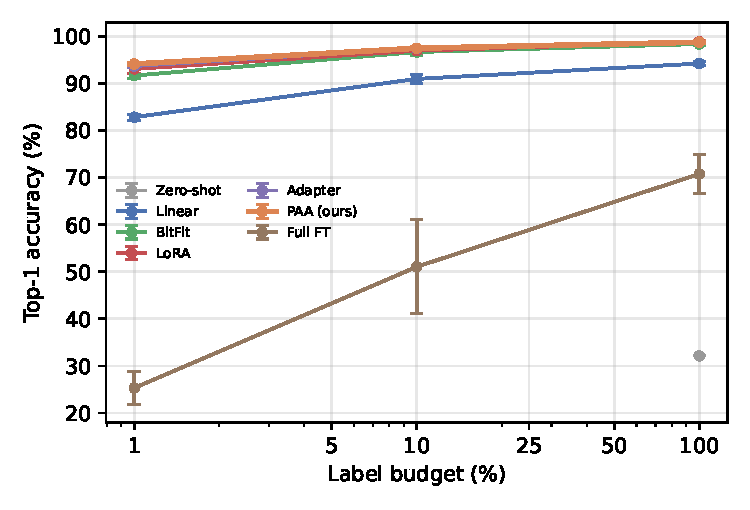
\includegraphics[width=0.48\textwidth]{figures/fig_curve_eurosat.pdf}\hfill
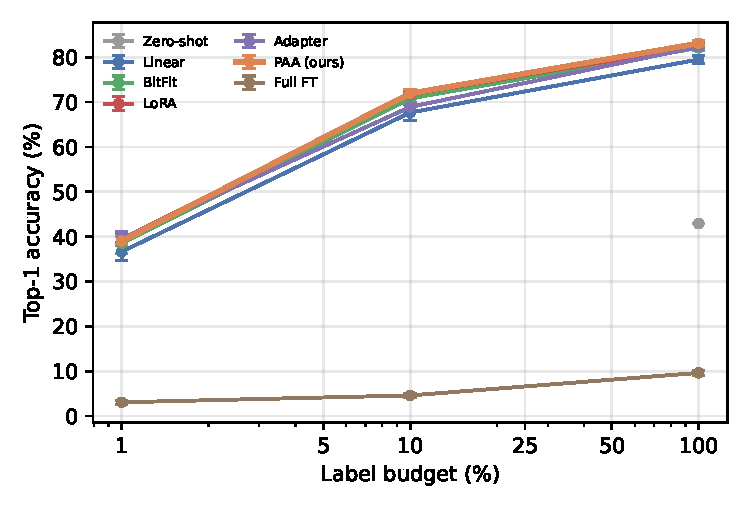
\includegraphics[width=0.48\textwidth]{figures/fig_curve_dtd.pdf}
\caption{Top-1 accuracy versus label budget on EuroSAT (left) and DTD (right),
CLIP ViT-B/16, shared-rate regime. Error bars denote standard deviation over three
seeds; zero-shot CLIP is 32.11\% and 42.91\% respectively.}
\label{fig:curve}
\end{figure}

What changes across datasets is where adaptation becomes worthwhile at all. On
EuroSAT even 216 images are enough for every parameter-efficient method to beat
zero-shot by more than 50 points; on DTD the same fraction leaves one image per
class and adaptation loses to doing nothing.

\subsection{Why the rate matters so much more for full fine-tuning}
\label{sec:lr}

Table~\ref{tab:lr-full} reports full fine-tuning on EuroSAT at $\rho=1\%$ across
the rates we ran, for all five backbones; Table~\ref{tab:lr-peft} does the same
for the parameter-efficient family on CLIP.

\begin{table}[t]
\centering
\caption{Full fine-tuning on EuroSAT at $\rho=1\%$: top-1 accuracy (\%) against the learning rate, mean over three seeds. Bold marks each backbone's best rate. Dashes are cells we did not run because the ViT optimum lies two orders of magnitude away from the convolutional one.}
\label{tab:lr-full}
\small
\setlength{\tabcolsep}{4pt}
\begin{tabular}{lccccccc}
\toprule
 & $10^{-5}$ & $3\times10^{-5}$ & $10^{-4}$ & $3\times10^{-4}$ & $10^{-3}$ & $3\times10^{-3}$ & $10^{-2}$ \\
\midrule
CLIP ViT-B/16 & \textbf{91.8} & 89.6 & 61.2 & 30.4 & 26.3 & -- & -- \\
ViT-B/16 (sup.) & 88.0 & \textbf{91.7} & 90.4 & 79.0 & 33.9 & -- & -- \\
ViT-S/16 (sup.) & 83.2 & 89.0 & \textbf{90.7} & 86.3 & 45.8 & -- & -- \\
ConvNeXt-T & 77.8 & 89.0 & 91.0 & \textbf{91.0} & 86.5 & 18.6 & 11.1 \\
ResNet-50 & 52.1 & 74.2 & 86.1 & \textbf{89.5} & 87.1 & 82.3 & 42.9 \\
\bottomrule
\end{tabular}
\end{table}

\begin{table}[t]
\centering
\caption{The parameter-efficient family on EuroSAT with CLIP at $\rho=1\%$: accuracy (\%) against the learning rate, mean over three seeds.}
\label{tab:lr-peft}
\small
\setlength{\tabcolsep}{4pt}
\begin{tabular}{lccc}
\toprule
 & $10^{-4}$ & $3\times10^{-4}$ & $10^{-3}$ \\
\midrule
Linear probe & 78.4 & 81.1 & \textbf{82.8} \\
BitFit & 83.4 & 88.1 & \textbf{91.8} \\
LoRA & 91.3 & 92.9 & \textbf{93.4} \\
Adapter & 92.8 & 92.4 & \textbf{94.0} \\
PAA & 91.4 & 92.9 & \textbf{94.2} \\
\bottomrule
\end{tabular}
\end{table}

Two facts stand out, and together they are the mechanism behind
\S\ref{sec:collapse}.

\paragraph{The optimum moves with the architecture} The best rate is $10^{-5}$ for
CLIP, $3\times10^{-5}$ for the supervised ViT-B, $10^{-4}$ for ViT-S and ConvNeXt,
and $3\times10^{-4}$ for ResNet-50. Between the two families the optimum moves by
one to two orders of magnitude, and it moves monotonically with architecture
within each family. For the parameter-efficient methods the best rate is always
$10^{-3}$, the top of their grid, so their optima lie at or above the largest
value we tried.

\paragraph{The sensitivity is much larger for full fine-tuning} Across the grid,
full fine-tuning spans 45 points on ViT-S, 58 on ViT-B, 66 on CLIP, 80 on
ConvNeXt and 47 on ResNet-50. The parameter-efficient family spans 1.6 to 8.4
points across three rates, and the ordering inside it never reverses. A single
rate is therefore a mild approximation for an adapter and a catastrophic one for
full fine-tuning, and where the shared rate sits determines which architecture
looks damaged.

The combination explains the left half of Table~\ref{tab:collapse} exactly: at
$10^{-3}$, full fine-tuning on CLIP is 65 points below its own best, while on
ResNet-50 it is within 2 points of its best. The apparent architectural
difference is the difference between two distances to two optima.

We can state this precisely and not explain it. The obvious candidate is that the
effective step size a transformer takes at a given nominal rate is larger than a
convolutional network's---attention and LayerNorm both rescale gradients---so the
same rate that is conservative for a ResNet is destructive for a ViT. Testing
that would need gradient-norm measurements per layer, which we did not take, and
we leave it open.

Two boundaries qualify the claim. CLIP's optimum is at the smallest rate we ran,
so 91.8 is a lower bound on what more tuning could reach; and the
parameter-efficient family's optimum is at the largest rate we ran, so its
figures are lower bounds in the opposite direction. Neither boundary affects the
comparison in Table~\ref{tab:collapse}, which uses each method's best value from
the rates actually run.

\subsection{Component ablation}
\label{sec:ablation}

Table~\ref{tab:ablation} isolates the two components of \ours, using a residual
adapter with a randomly initialized head and no anchoring term as the reference.
The rows are separate runs: the reference at $\rho=1\%$ sits at 92.49 here against
93.69 for the same configuration in Table~\ref{tab:eurosat}, a difference of 1.2
points that is inside the run-to-run variation of \S\ref{sec:metrics}. We therefore
compare variants within this table and not against Table~\ref{tab:eurosat}.

\begin{table}[t]
\centering
\caption{Ablation of the two components of \ours\ on EuroSAT with CLIP (top-1
\%, three seeds).}
\label{tab:ablation}
\small
\setlength{\tabcolsep}{6pt}
\begin{tabular}{lcc}
\toprule
Variant & $\rho=1\%$ & $\rho=10\%$ \\
\midrule
Adapter only              & 92.49$\pm$1.43 & 97.10$\pm$0.37 \\
\quad + prototypical init & 93.15$\pm$0.38 & 97.53$\pm$0.34 \\
\quad + anchoring         & 94.02$\pm$0.67 & 96.98$\pm$0.14 \\
\textbf{\ours} (both)     & 93.88$\pm$1.15 & 97.59$\pm$0.16 \\
\bottomrule
\end{tabular}
\end{table}

At $\rho=1\%$ the anchoring term alone raises accuracy from 92.49\% to 94.02\%
($+1.53$), the largest single effect inside this ablation, although
the standard deviations of the two conditions overlap. Prototypical
initialization alone raises accuracy to 93.15\% ($+0.66$) and, more clearly,
reduces the seed-to-seed standard deviation from 1.43 to 0.38. The two
components do not compose additively: the full method reaches 93.88\%, the same
as anchoring alone within run-to-run variation. At $\rho=10\%$ all four variants
lie within 0.61 points and the ordering is not stable. Every contrast here is
smaller than 1.6 points, and identical configurations can differ by 1.4, so we
read the table as weak but consistent evidence that the anchoring term does most
of the work rather than as a decomposition.

We therefore attribute the low-budget behaviour of \ours\ mainly to the
anchoring term, and regard prototypical initialization as a stabilizer rather
than an independent source of accuracy. We report this as measured rather than
selecting the variant that looks best at a single seed.

\subsection{Efficiency}

Table~\ref{tab:efficiency} reports trainable parameters and training time at
$\rho=100\%$ on EuroSAT with CLIP.

\begin{table}[t]
\centering
\caption{Efficiency on EuroSAT with CLIP at $\rho=100\%$ (one RTX 5070~Ti
laptop GPU, three seeds).}
\label{tab:efficiency}
\small
\setlength{\tabcolsep}{6pt}
\begin{tabular}{lccc}
\toprule
Method & \#Trainable & Train time (min) & GPU hours \\
\midrule
Linear probe & 0.01M & 5.7 & 0.3 \\
BitFit       & 0.18M & 15.0 & 0.8 \\
LoRA         & 1.33M & 18.7 & 0.9 \\
Adapter      & 5.40M & 20.8 & 1.0 \\
\textbf{\ours} & 5.40M & 20.1 & 1.0 \\
Full FT      & 149.63M & 18.8 & 0.9 \\
\bottomrule
\end{tabular}
\end{table}

Restricting the update to a few million parameters does not reduce wall-clock
time in proportion, because gradients must still be back-propagated through the
frozen backbone; the saving is in optimizer state and model storage rather than
in the forward--backward pass. The practical argument for the adapter family is
therefore accuracy and stability, not speed. \ours\ adds no inference cost at
all: its prototypes and anchoring term are used only during training.

\subsection{Class-balanced behaviour}

Macro-averaged accuracy tracks top-1 within 0.2 points for every
parameter-efficient method, so the ranking above is not an artefact of class
imbalance. The exception is full fine-tuning on CLIP at the shared rate, where macro
accuracy is 2.2 points below top-1 at $\rho=1\%$ (23.12\% against 25.30\%),
indicating that the classes it retains are the ones with the largest training
subsets; at the tuned rate the gap closes to 0.4 points.

%% ============================================================================
\section{Discussion}
\label{sec:discussion}

\subsection{What the shared-rate comparison was measuring}

The left half of Table~\ref{tab:collapse} is the result we expected to build a
paper on: two ViTs of identical architecture, trained with different objectives,
failing in the same way, while convolutional backbones of comparable and smaller
size do not fail. A pattern like that invites an architectural explanation, and we
developed two candidates for it---the loss of explicit locality priors, and a
gradient path that moves every layer at once.

The right half of the same table makes both explanations unnecessary. Once each
method is trained at a rate chosen on the validation split, the family difference
on EuroSAT is 2.6 points at worst and the identity of the best method changes from
cell to cell. Nothing in the tuned data requires an architectural account, and we
do not add one.

What the shared-rate comparison measures is each architecture's sensitivity to a
nominal rate. ViTs are more sensitive than CNNs by one to two orders of magnitude
in the rate that maximises accuracy, and full fine-tuning is more sensitive than
any parameter-efficient method. A comparison that fixes the rate at a value
convenient for one end of that spectrum reports the distance to the other end's
optimum and calls it an architectural property.

This does not make the sensitivity a nuisance to be tuned away. Two consequences
are real. The sensitivity is itself a property of the architecture worth knowing:
a practitioner who inherits a rate from a convolutional recipe and applies it to a
ViT reproduces our left-hand column. And the tuned column costs a search that most
studies, and most practitioners with a few hundred labels, will not run.

\subsection{What a practitioner should do}

Given a few hundred labels and a frozen encoder, the numbers suggest four checks,
in this order.

Measure zero-shot first. On both datasets it is a real baseline, and on DTD at one
example per class it is the best option available.

Count examples per class, not the fraction. At one or two per class adaptation
loses to doing nothing even with a tuned rate, and the effort is better spent on
labels.

If adaptation is warranted, start with a linear probe and an adapter: the adapter
buys 10.9 points over the probe with CLIP, 3.4 with the supervised ViT and 5.8
with ResNet-50 at the shared rate, and it does so without a tuning search. Full
fine-tuning is worth considering only if you are prepared to tune its rate, in
which case it matches the adapter family on EuroSAT and stays 3--10 points behind
it on DTD.

Finally, and most importantly, do not inherit a learning rate across
architectures. The single largest error we measured is not the choice of method
but the choice of rate: 66 points for full fine-tuning on CLIP between the worst
and best value, against 1.6--8.4 points for the whole parameter-efficient family.
If the rate must be fixed, fix it after one short validation sweep on the target
architecture, not before.

\subsection{Threats to validity}
\label{sec:threats}

\emph{One hyperparameter, two regimes.} Our correction rests on a single
intervention, the learning rate. We did not vary warm-up, layer-wise decay or
batch size, and it remains possible that a different intervention would produce a
different picture---one in which neither regime is the right description. The
claim we defend is narrow: at the settings we ran, the architectural difference
disappears when the rate is tuned, and we have no evidence that a third
intervention would bring it back.

\emph{Two datasets.} A domain with different label-noise characteristics could
change the ordering within the adapter family, whose members differ by less than
the noise floor.

\emph{Grid boundaries.} Two of the five optima sit at the edge of the grid we ran:
CLIP's best rate is the smallest we tried, and the parameter-efficient family's
best rate is the largest. The tuned numbers are therefore lower bounds on both
sides, by an unknown amount, and a wider grid in either direction would move them.
The comparison in Table~\ref{tab:collapse} uses each method's best value from the
rates actually run, so it is internally consistent, but it is not the last word on
how well any of these methods can do.

\emph{Two points on the examples-per-class axis.} Our budgets place 1 and 22
examples per class on EuroSAT and 1 and 10 on DTD. The claim that the number of
examples per class governs the outcome therefore rests on the contrast between a
single example and a couple of dozen, with nothing in between.

\emph{Incomplete grids.} Four of the five backbones were evaluated at the two
scarce budgets only, so their entries have no full-data counterpart in
Tables~\ref{tab:eurosat} and~\ref{tab:dtd}. The paper's question concerns the
scarce regime, but the omission should be visible.

\emph{Statistical power and repeat noise.} With three seeds a paired $t$-test has
low power, and we use it as a secondary check rather than as the primary evidence;
the single significant result against \ours\ is supported by a consistent sign
across all three seeds, which is the more informative fact. More consequentially,
repeating identical configurations changes accuracy by up to 1.4 points
(\S\ref{sec:metrics}), which is larger than several of the differences we report.
Where a difference is of that size we now say so in place, but a reader should
treat sub-point orderings anywhere in the tables as unresolved.

\emph{Remedies we did not test.} Three standard ways of letting a transformer
take a larger effective step are absent from the grid: warm-up, layer-wise
learning-rate decay, and the two-stage probe-then-fine-tune recipe of
\cite{kumar2022finetuning}. Any of them would plausibly move the tuned numbers
further up, so the tuned column should be read as what a plain learning-rate
search achieves, not as the ceiling for these architectures.

\emph{Scope of the regularizer.} The anchoring term needs class prototypes, and so
presumes at least one labelled example per class. That holds in our protocol but
not in open-set or truly zero-shot settings.

\section{Conclusion}
\label{sec:conclusion}

We set out to explain why published comparisons disagree about whether full
fine-tuning is worth it under label scarcity, and we found an answer that
invalidated our own hypothesis. Across eight adaptation paradigms, five backbones
and two datasets, run twice---once with one shared learning rate and once with the
rate chosen per method---the disagreement turns out to be reproducible from the
protocol alone.

With every method at $10^{-3}$, the transformer backbones lose 8--69 points to the
best parameter-efficient method and the convolutional ones lose at most 15. The
pattern is clean enough to support an architectural story, and we built one. With
the rate chosen on the validation split, the same cells show the three transformer
backbones within 2.6 points of the best parameter-efficient method on EuroSAT, and
the CLIP gap falls from 68.8 to 2.3. The architectural story does not survive, and
we withdraw it here.

The mechanism is measurable and simple. The rate that maximises accuracy differs
by one to two orders of magnitude between full fine-tuning on a ViT and on a CNN,
and full fine-tuning spans 45--80 points across the grid where the whole
parameter-efficient family spans 1.6--8.4. A shared rate is a mild approximation
for an adapter and a decisive one for full fine-tuning, so the rate a study
happens to inherit largely determines which architecture it reports as fragile.

Two results are unaffected by the correction. At one labelled image per class,
nothing beats zero-shot, and full fine-tuning stays 3--10 points behind the
parameter-efficient family---the one place where a real deficit remains, and it
belongs to the budget rather than to the architecture. And within the
parameter-efficient family the ordering is stable, with adapter and LoRA ahead of
BitFit and the linear probe, and prompt learning the weakest adapted method under
this protocol.

The prototype-anchored variant we proposed is competitive and never significantly
better; the one significant paired difference in the grid goes against it. We
report it, its ablation and its cost, and claim nothing more.

Every statement above is conditional, and the conditions are now mostly about
ranges of hyperparameters rather than about architectures. Code, splits, all
1{,}428 configurations and the selection script are released so that the
conditions can be re-checked and extended.

\appendix
\section{Per-method results for the two additional backbones}
\label{app:extra}

Tables~\ref{tab:app-vits} and~\ref{tab:app-convnext} report the complete grid for
the two backbones used to break the parameter-count confound. Means over three
seeds; standard deviations are omitted for space and are available with the
released results.

\begin{table}[h]
\centering
\caption{ViT-S/16 (supervised, 21.7M), shared-rate regime: top-1 accuracy (\%),
mean over three seeds. CoOp is defined only for the image--text backbone.}
\label{tab:app-vits}
\small
\setlength{\tabcolsep}{6pt}
\begin{tabular}{lcccc}
\toprule
 & \multicolumn{2}{c}{EuroSAT} & \multicolumn{2}{c}{DTD} \\
\cmidrule(lr){2-3}\cmidrule(lr){4-5}
Method & 1\% & 10\% & 1\% & 10\% \\
\midrule
CoOp & -- & -- & -- & -- \\
Linear probe & 86.54 & 91.73 & 28.01 & 55.38 \\
BitFit & 88.93 & 95.85 & 28.25 & 59.46 \\
LoRA & 90.77 & 97.17 & 27.54 & 59.63 \\
Adapter & 90.83 & 97.12 & 27.60 & 59.87 \\
\ours & 91.44 & 96.96 & 26.24 & 61.05 \\
Full FT & 45.75 & 89.16 & 12.17 & 15.90 \\
\bottomrule
\end{tabular}
\end{table}

\begin{table}[h]
\centering
\caption{ConvNeXt-T (28.6M), shared-rate regime: top-1 accuracy (\%), mean over
three seeds.}
\label{tab:app-convnext}
\small
\setlength{\tabcolsep}{6pt}
\begin{tabular}{lcccc}
\toprule
 & \multicolumn{2}{c}{EuroSAT} & \multicolumn{2}{c}{DTD} \\
\cmidrule(lr){2-3}\cmidrule(lr){4-5}
Method & 1\% & 10\% & 1\% & 10\% \\
\midrule
CoOp & -- & -- & -- & -- \\
Linear probe & 89.32 & 94.43 & 32.51 & 63.71 \\
BitFit & 91.30 & 96.62 & 31.91 & 64.78 \\
LoRA & 90.53 & 96.91 & 32.62 & 65.54 \\
Adapter & 91.96 & 96.88 & 33.39 & 64.89 \\
\ours & 92.27 & 97.14 & 32.68 & 66.61 \\
Full FT & 86.49 & 96.38 & 26.12 & 51.36 \\
\bottomrule
\end{tabular}
\end{table}

\section*{CRediT authorship contribution statement}
\textbf{Jiahao Wu:} Conceptualization, Methodology, Software, Investigation,
Formal analysis, Writing -- original draft. \textbf{Sihao Li:} Validation, Data
curation, Visualization, Writing -- review and editing.

\section*{Declaration of generative AI and AI-assisted technologies in the
writing process}
During the preparation of this work the authors used Claude and DeepSeek to
assist with language editing and with the implementation of parts of the
experimental code. After using these tools, the authors reviewed and edited the
content and verified all reported results, and they take full responsibility for
the content of the publication.

\section*{Declaration of competing interest}
The authors declare that they have no known competing financial interests or
personal relationships that could have appeared to influence the work reported
in this paper.

\section*{Data availability}
The datasets used are public (EuroSAT and DTD). Code, split files and all
configuration files are available at
\url{https://github.com/REPLACE-ME/REPLACE-ME}.
% TODO(作者)：把上面网址里的两个 REPLACE-ME 换成你的 GitHub 用户名和仓库名，
% 然后删掉这行注释和下一行。
% 例：\url{https://github.com/jiahaowu/paa-label-scarcity}

\bibliographystyle{elsarticle-num}
\bibliography{refs}

\end{document}
